%% LyX 2.0.5.1 created this file.  For more info, see http://www.lyx.org/.
%% Do not edit unless you really know what you are doing.
\documentclass[english]{article}
\usepackage[T1]{fontenc}
\usepackage[latin9]{inputenc}
\usepackage{graphicx}
\usepackage{babel}
\begin{document}
\begin{figure}
\begin{centering}
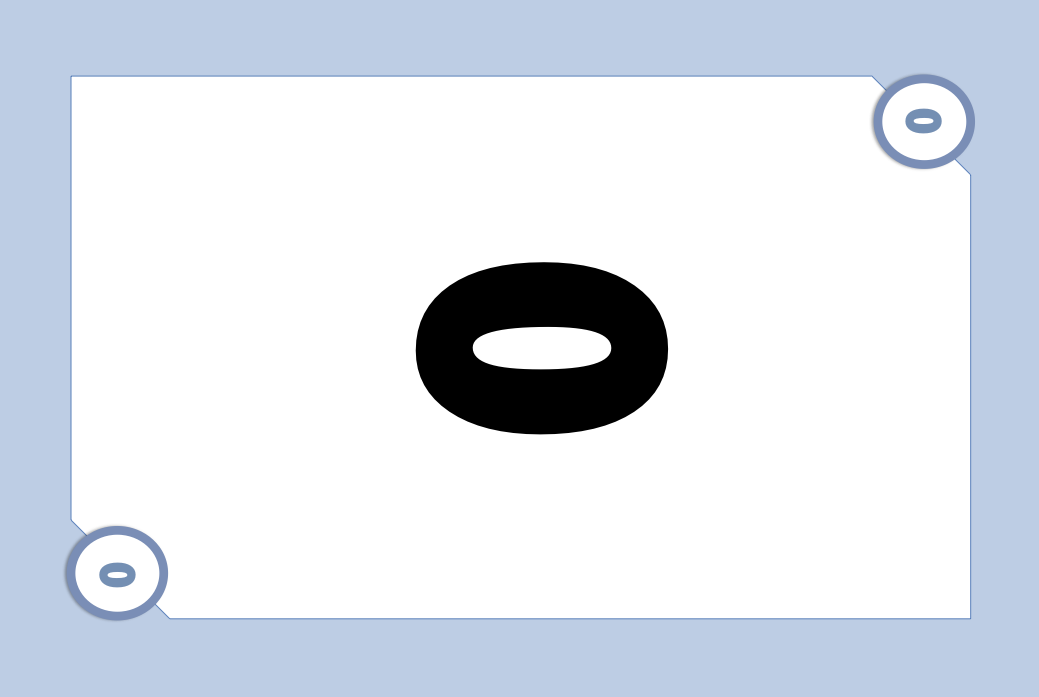
\includegraphics[angle=90,scale=0.5]{side-A/b-0}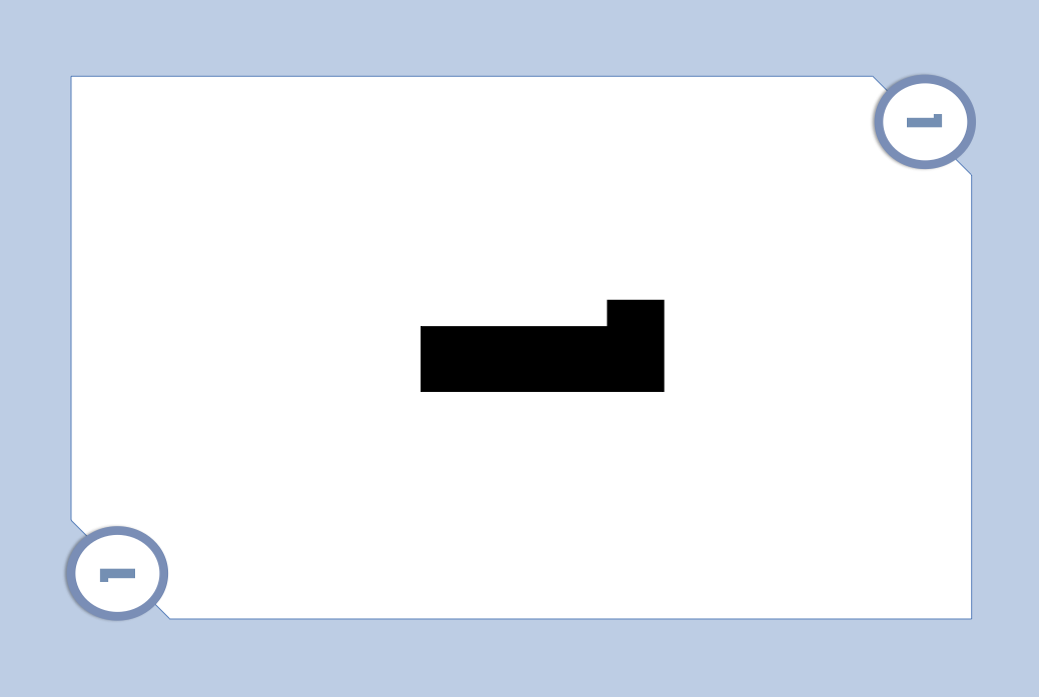
\includegraphics[angle=90,scale=0.5]{side-A/b-1}
\includegraphics[angle=90,scale=0.5]{side-A/b-2}
\includegraphics[angle=90,scale=0.5]{side-A/b-3}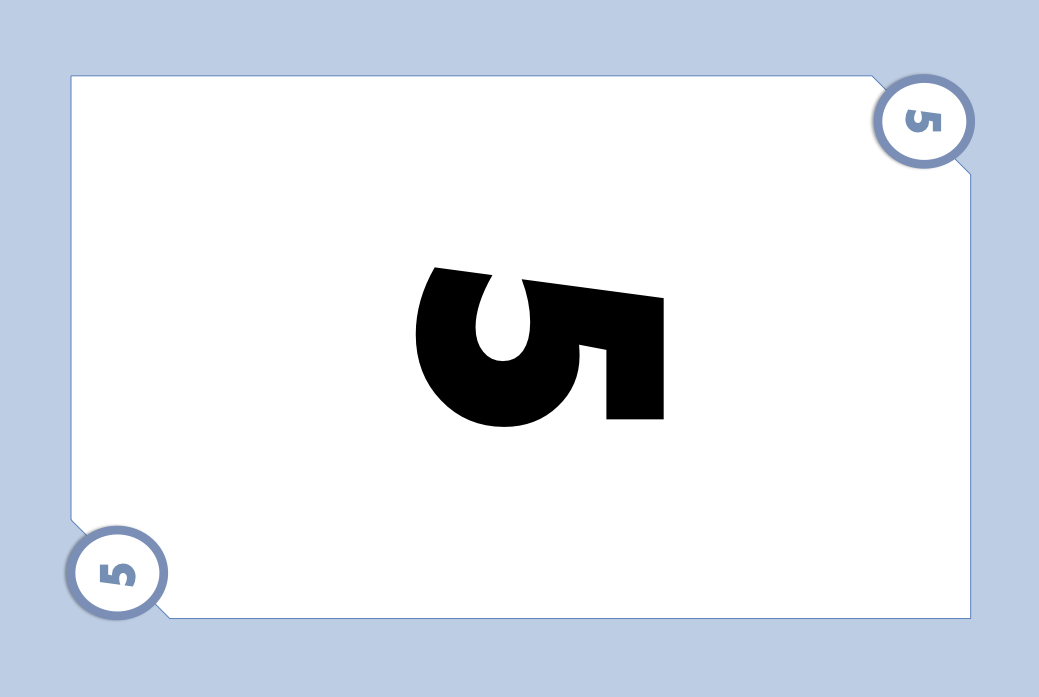
\includegraphics[angle=90,scale=0.5]{side-A/b-5}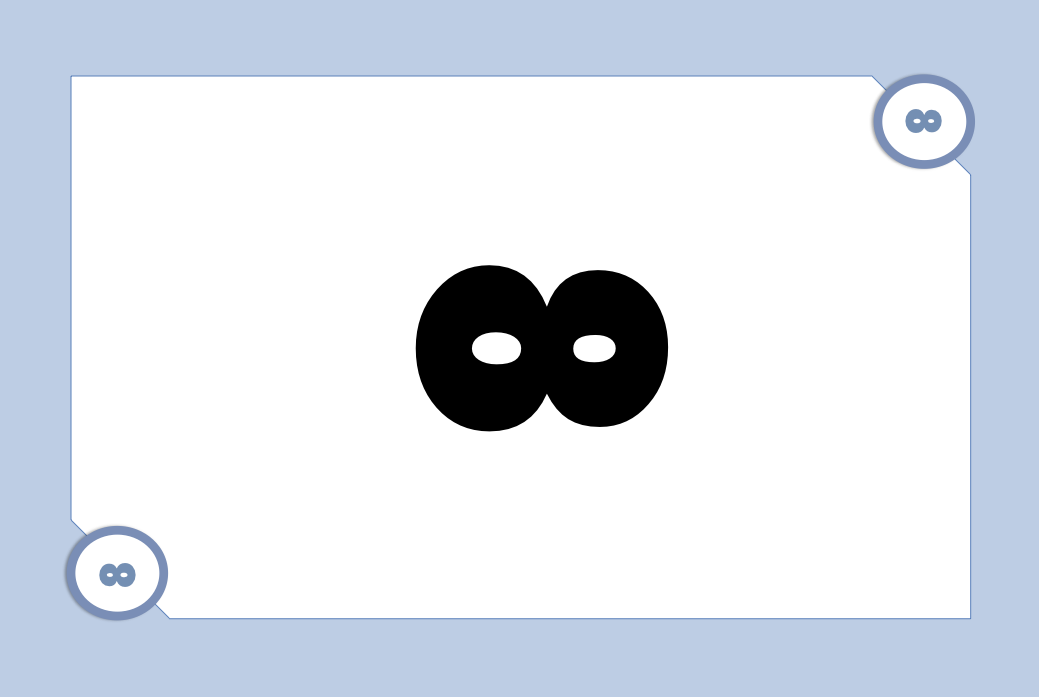
\includegraphics[angle=90,scale=0.5]{side-A/b-8}
\par\end{centering}

\begin{centering}
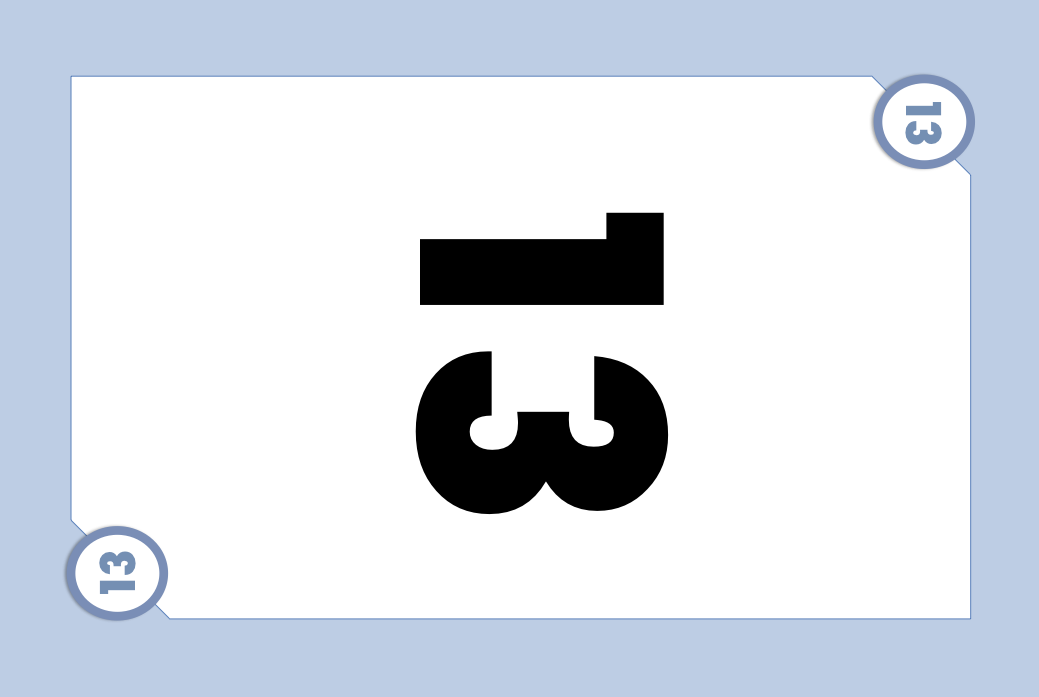
\includegraphics[angle=90,scale=0.5]{side-A/b-13}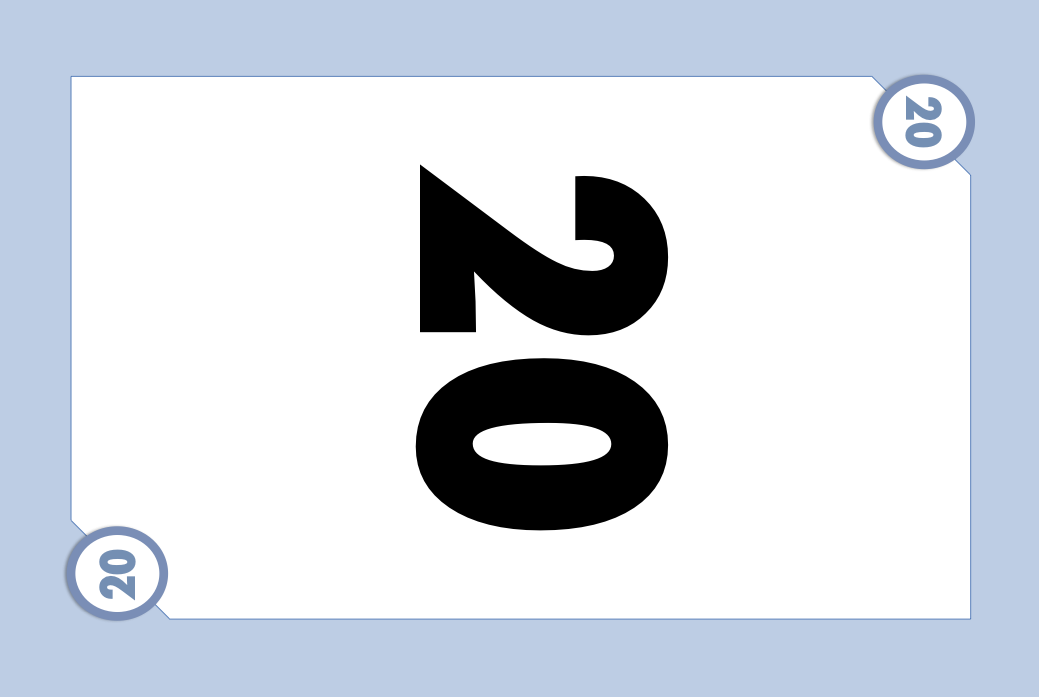
\includegraphics[angle=90,scale=0.5]{side-A/b-20}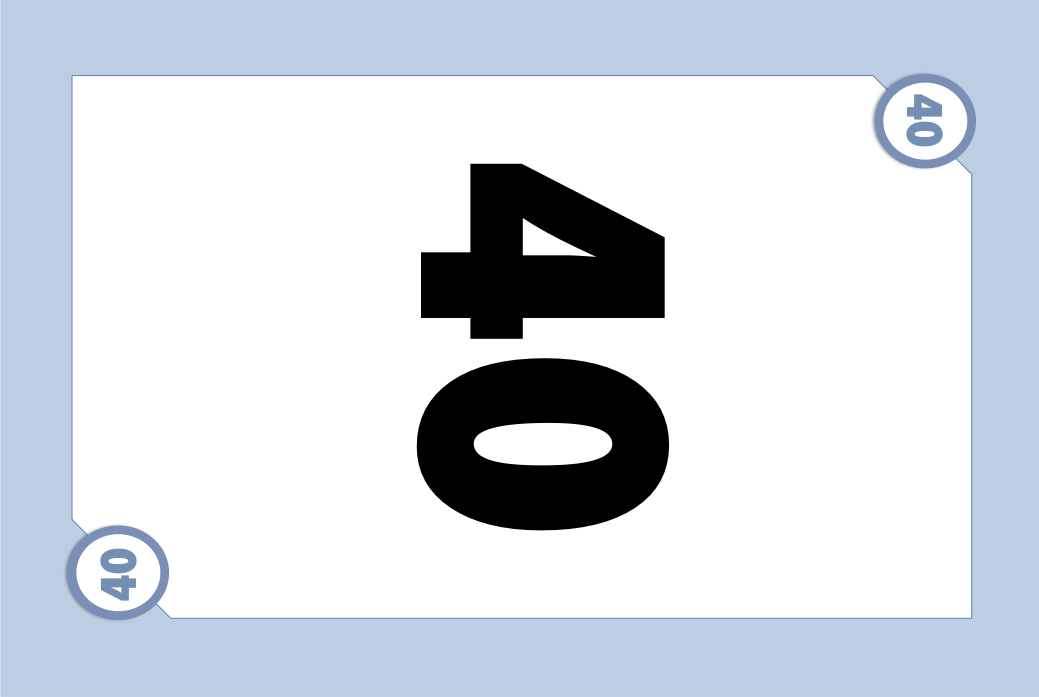
\includegraphics[angle=90,scale=0.5]{side-A/b-40}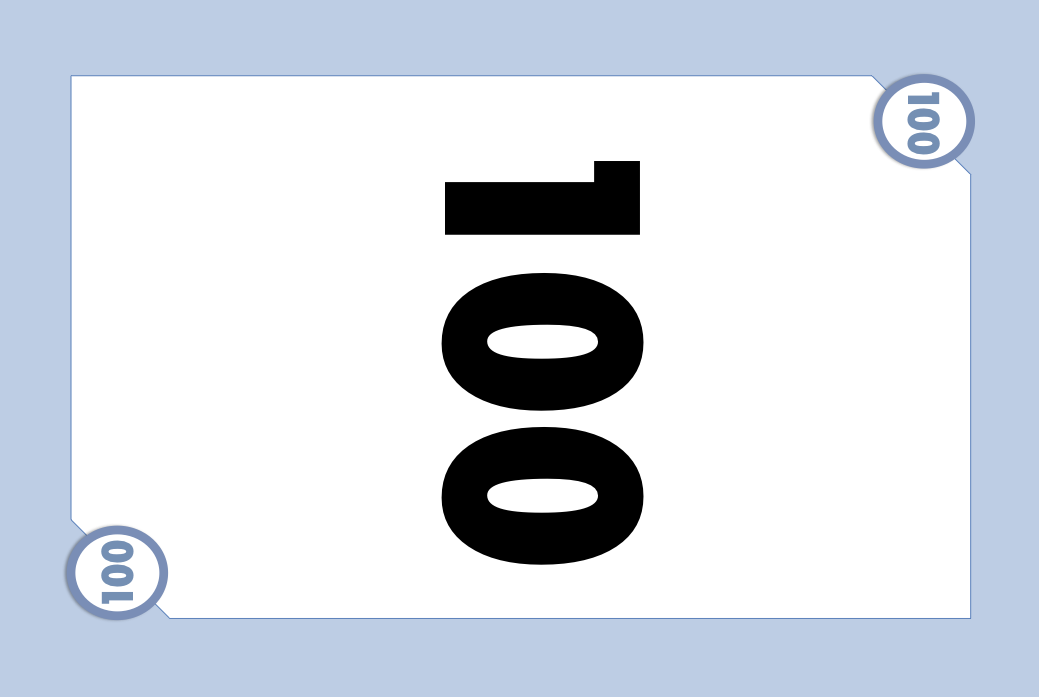
\includegraphics[angle=90,scale=0.5]{side-A/b-100}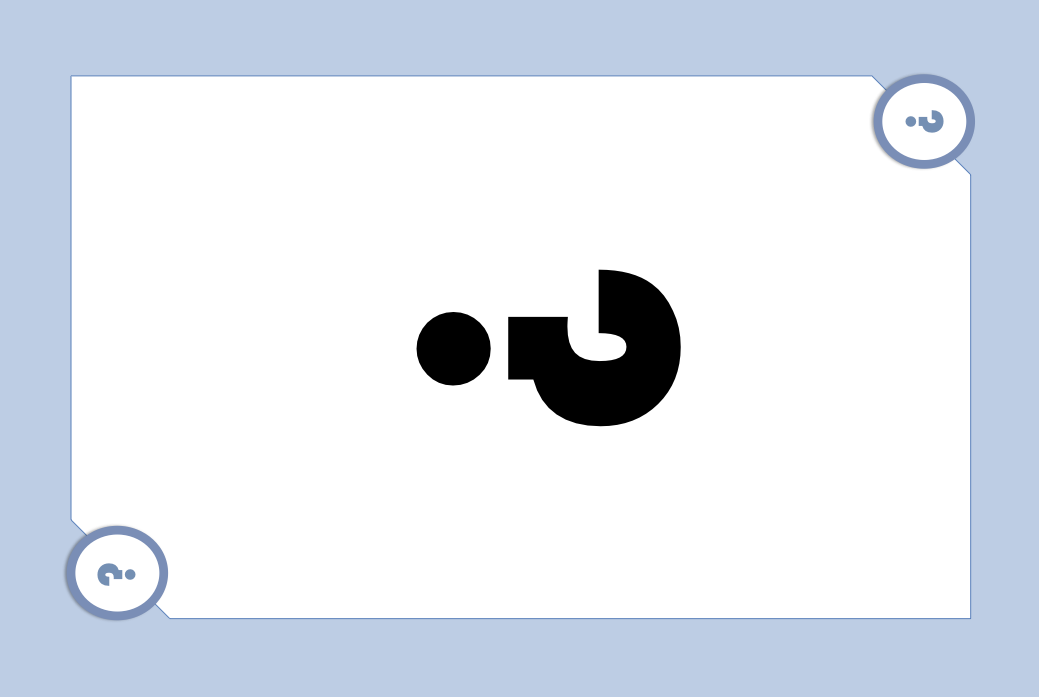
\includegraphics[angle=90,scale=0.5]{side-A/b-noidea}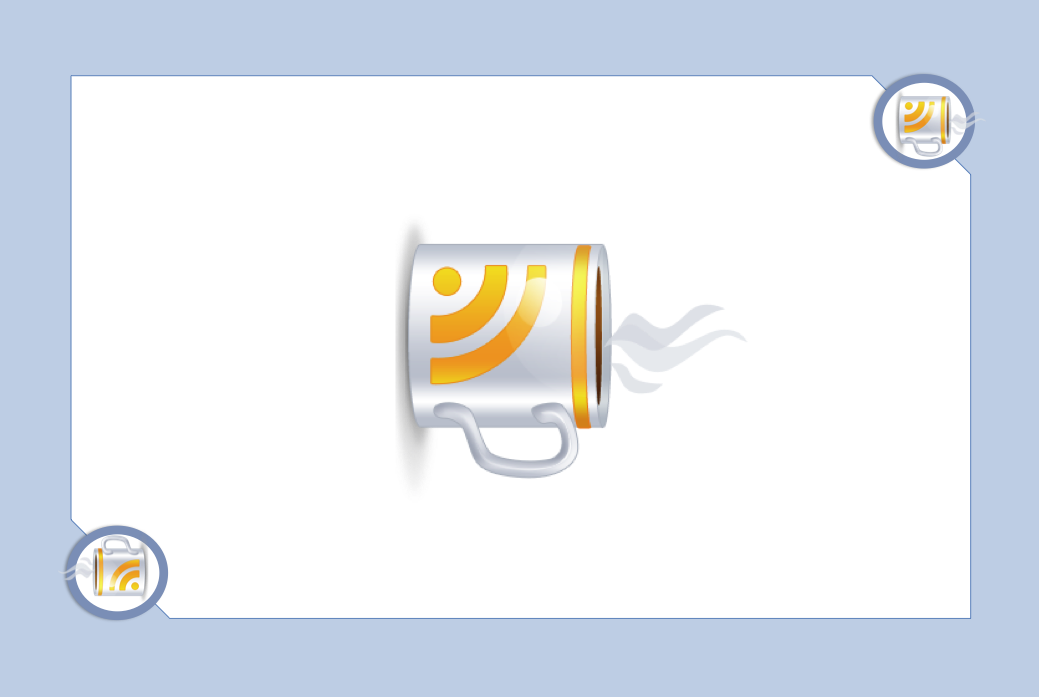
\includegraphics[angle=90,scale=0.5]{side-A/b-coffee}
\includegraphics[angle=90,scale=0.5]{side-A/g-1}
\includegraphics[angle=90,scale=0.5]{side-A/g-8}
\par\end{centering}

\caption{}


\end{figure}

\end{document}
